\subsection{Multilevel converter}
\label{sec:cap4:multilevel-converter}

\subsubsection{Parameters of the Simulation}

This example describes the Multilevel converter model described in session \ref{sec:cap2:multilevel-converter},
the dynamics of this system are defined by 

\begin{equation}
    \begin{matrix}
        A_i = \left[ 
            \begin{matrix} 
                0 &       0 & \Big(u_2(i)-u_1(i)\Big)/C1 \\ 
                0 & 0 & \Big(u_3(i)-u_2(i)\Big)/C2 \\ 
                \Big(u_1(i)-u_2(i)\Big)/L & \Big(u_2(i)-u_3(i)\Big)/L & -R/L \\ 
            \end{matrix} \right] \\
            \\
        b_i = \left[ \begin{matrix} 0 \\ 0 \\ \Big(E/L\Big) u_3(i) \end{matrix} \right]
    \end{matrix}
\end{equation}

\noindent
with \highlight{$R = 10.0 \; \mathrm{\Omega}$}, \highlight{$L = 10.0 \; \mathrm{mH}$}, \highlight{$C_1 = 40.0 \; \mathrm{\mu F}$}, 
\highlight{$C_2 = 40.0 \; \mathrm{\mu F}$}, \highlight{$E  = 30.0 \; \mathrm{V}$}

\noindent
and the associated mode sequence for the target cyclic trajectory is shown in Figure \ref{fig:cap4:multilevel-converter-reference-sequence}.

\begin{figure}[H]
    \centering
    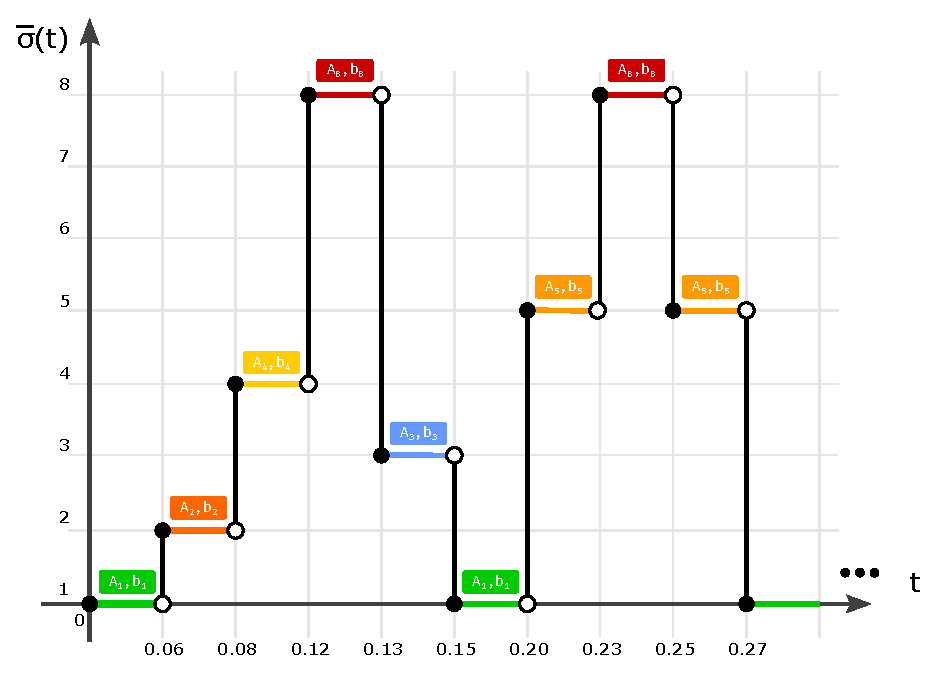
\includegraphics[width=12cm]{figures/shared/cap4_ref_signal_patino2.eps}
    \caption{Reference sequence for Multilevel converter}
    \label{fig:cap4:multilevel-converter-reference-sequence}
\end{figure}

\noindent
with \highlight{$u(i)$} given in Table \ref{tab:cap4:multilevel-converter-input-values} 

\noindent
\begin{table}[H]
    \caption{Values of $u_i$ for the Multilevel converter}
    \label{tab:cap4:multilevel-converter-input-values}
    \begin{center}
        \begin{tabular}{|c|c|c|c|}
            \hline
                \textbf{mode (i)}   & \boldmath{$u_1$} & \boldmath{$u_2$} & \boldmath{$u_3$} \\
            \hline
                1 & 0 & 0 & 0 \\
                2 & 0 & 0 & 1 \\
                3 & 0 & 1 & 0 \\
                4 & 0 & 1 & 1 \\
                5 & 1 & 0 & 0 \\
                6 & 1 & 0 & 1 \\
                7 & 1 & 1 & 0 \\
                8 & 1 & 1 & 1 \\
            \hline
        \end{tabular}
    \end{center}
\end{table}



\noindent
and the operation mode is characterized by the index \highlight{$\Omega = \big[1,2,4,8,3,1,5,8,5\big]$}. 
The time switch values are defined as \highlight{$\tau^\infty = \big[0, 0.0639, 0.0878, 0.1119, 0.1344, 0.1567, 0.2065, $} 
\highlight{$0.23, 0.2529, 0.2756\big] \; \mathrm{ms}$}, and the reference state vector for this 
trajectory is denoted as \highlight{$\bar{x}_{ref} = \big[10 \;\mathrm{V}, 20 \;\mathrm{V}, 1 \;\mathrm{A}\big]$}. Additionally, the 
maximum period value for the trajectory cycle is specified as \highlight{$T_{p_{max}} = 4\times 10^{-4} $}, 
while the initial state of the nominal target trajectory is given by \highlight{$x_0 = \big[9.5143 \;\mathrm{V}, 19.8211 \;\mathrm{V}, 1.0314 \;\mathrm{A}\big]$}. 
The time step of the simulation is \highlight{$t_{step} = 1 \times 10^{-7} \;\mathrm{s}$} and the weight matrix used in the 
computation of the trajectory is \highlight{$Q = diag([10, 5, 20000])$}.

\subsubsection{Prediction Matrices}

The prediction matrices are constructed using  \eqref{eq:cap4:linearization-phi} and \eqref{eq:cap4:linearization-gamma}, and the result is

\begin{equation}
    \Phi =
    \left[
    \begin{matrix}
       0.999539  &   0.001900 & -0.124610 \\
      -0.002031  &   0.999915 &  0.000764 \\
      -0.000461  &  -0.000290 &  0.759578
    \end{matrix}
    \right]
\end{equation}

\begin{equation}
    \Gamma =
    \left[
    \begin{matrix}
         0.007784  &  -2.578391  &  -0.081618 \\
        -2.400410  &   2.472097  &  -0.079094 \\
         2.477894  &   0.042370  &  -0.076050 \\
        -2.602774  &   2.388977  &   0.171509 \\
         2.472432  &  -2.594318  &   0.102211 \\
         2.703328  &       0     &  -0.087828 \\
        -2.354659  &       0     &  -0.189865 \\
         2.354483  &       0     &   0.199932
    \end{matrix}
    \right]^T
    \times 10^4
\end{equation}

\noindent
with the switching time constraints

\begin{equation}
    c = 
    \left[
        \begin{matrix}
            -\Delta t_{r_1} +\Delta t_{r_{1, min}} \\
            -\Delta t_{r_2} +\Delta t_{r_{2, min}} \\
            \vdots \\
            -\Delta t_{r_{N-1}} +\Delta t_{r_{{N-1}, min}} \\
            -\Delta t_{r_N} +\Delta t_{r_{N, min}} \\
        \end{matrix}
    \right] = 
    \left[
        \begin{matrix}
            -0.638811 + 0.20 \\
            -0.239318 + 0.20 \\
            -0.240440 + 0.20 \\
            -0.225094 + 0.20 \\
            -0.223339 + 0.20 \\
            -0.497696 + 0.20 \\
            -0.235714 + 0.20 \\
            -0.228086 + 0.20 \\
            -0.227575 + 0.20
        \end{matrix}
    \right] \times 10^{ -4  }=
    \left[
        \begin{matrix}
            -0.438811 \\
            -0.039318 \\
            -0.040440 \\
            -0.025094 \\
            -0.023339 \\
            -0.297696 \\
            -0.035714 \\
            -0.028086 \\
            -0.027575
        \end{matrix}
    \right] \times 10^{ -4 }
\end{equation}

\subsubsection{Results}


Figure \ref{fig:cap4:multilevel-converter-feasibility-region} presents the feasibility region $\mathcal{D}$ for three different prediction horizons 
($N_p = 1$, $N_p = 2$ and $N_p = 4$) for the Multilevel Converter.


\begin{figure}[H]
    \centering
    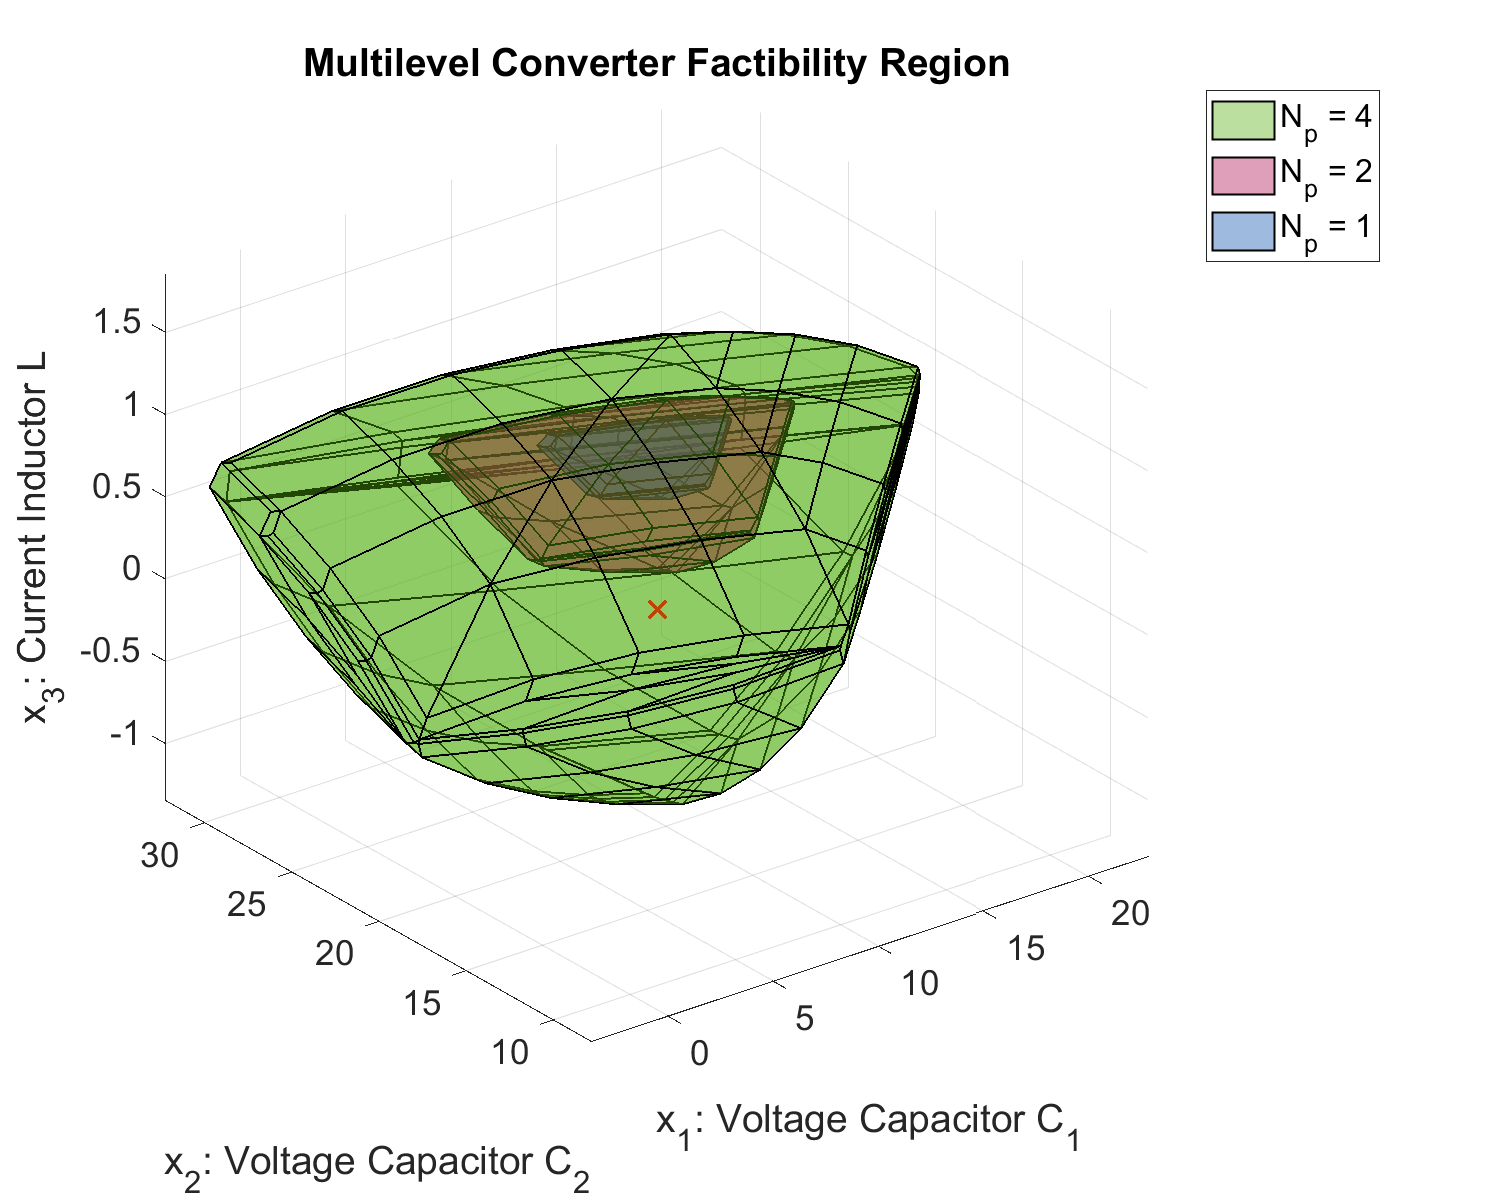
\includegraphics[width=14cm]{figures/cap4/graf_proj_patino2.pdf}
    \caption{Multilevel Converter: Feasibility Region}
    \label{fig:cap4:multilevel-converter-feasibility-region}
\end{figure}


Figure \ref{fig:cap4:multilevel-converter-state-trajectory-a} shows the trajectory for the Multilevel converter, 
\highlightblue{in blue} we see the trajectory without using the MPC controller, and 
\highlightorange{in orange} we see the trajectory using the MPC controller.
Both trajectories start from \highlight{$x_0 = \big[7.5143 \;\mathrm{V}, 20.8211 \;\mathrm{V}, 0.0314 \;\mathrm{A}\big]$}.
The trajectory with the MPC off drifts away from the desired behavior, 
converging to a different limit cycle. However, the trajectory with the MPC on
successfully drives the system to the target position \highlight{$\bar{x}_0 = \big[9.5143 \;\mathrm{V}, $} \highlight{$19.8211 \;\mathrm{V}, 1.0314 \;\mathrm{A}\big]$}.
It is important to note that \highlight{$\bar{x}_0$} represents the initial condition of the target cyclic trajectory;
therefore, converging to this point is equivalent to converging to the desired limit cycle.


\begin{figure}[H]
    \centering
    
\includegraphics[width=14cm]{figures/cap4/graf_patino2_traj.pdf}
    \caption{Multilevel Converter: State Trajectory, $x_0 = \big[7.51, 20.82, 0.03\big]^T$}
    \label{fig:cap4:multilevel-converter-state-trajectory-a}
\end{figure}

Note that the trajectory of Figure \ref{fig:cap4:multilevel-converter-state-trajectory-a} does not converge to the same periodic trajectory.
In Figure \ref{fig:cap4:multilevel-converter-state-trajectory-b} we run the simulation with a different initial condition \highlight{$x_0$} and we see 
that the trajectory with the MPC turned off converges to yet another periodic trajectory.

\begin{figure}[H]
    \centering
    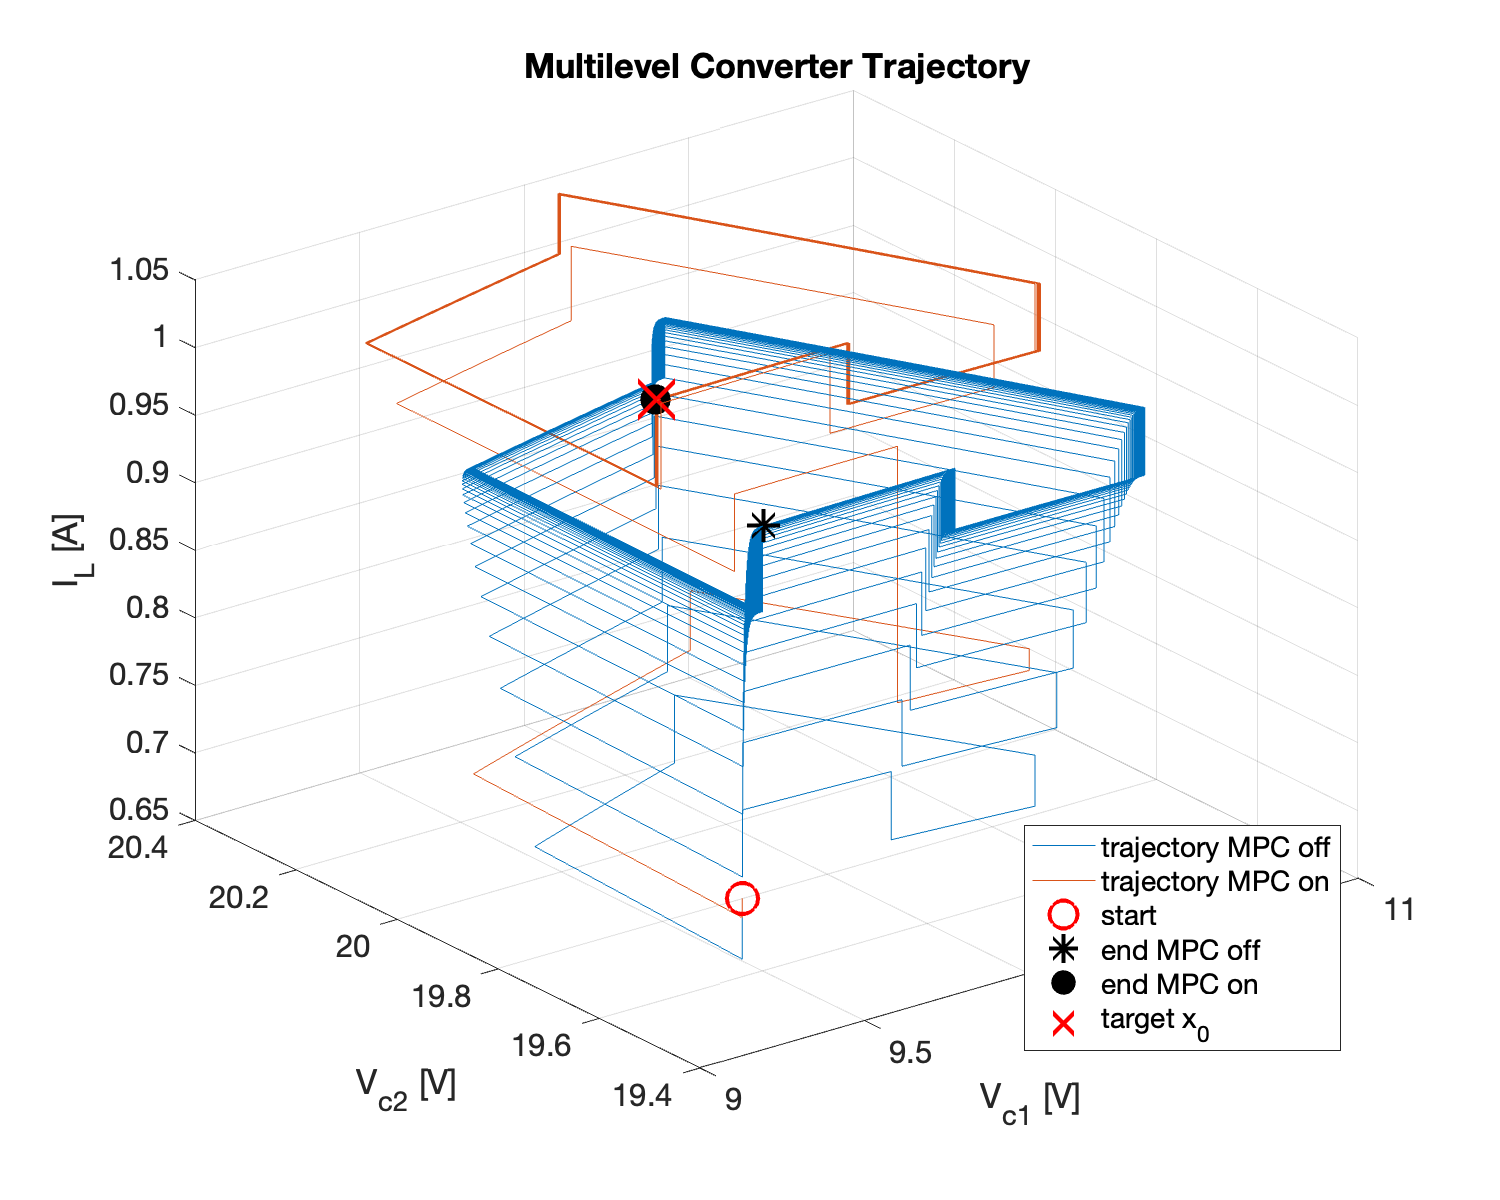
\includegraphics[width=14cm]{figures/cap4/graf_patino2_traj_2.pdf}
    \caption{Multilevel Converter: State Trajectory, $x_0 = \big[9.31, 19.52, 0.73\big]^T$}
    \label{fig:cap4:multilevel-converter-state-trajectory-b}
\end{figure}

Figure \ref{fig:cap4:multilevel-converter-states} displays the states of the system over time.

\begin{figure}[H]
    \centering
    
\includegraphics[width=14cm]{figures/cap4/graf_patino2_xi.pdf}
    \caption{Multilevel Converter: States over time}
    \label{fig:cap4:multilevel-converter-states}
\end{figure}

Figure \ref{fig:cap4:multilevel-converter-control-signal} displays the control signal sequence, 
we can see the difference between the open loop and the controlled signal decreasing
and getting in sync.

\begin{figure}[H]
    \centering
    
\includegraphics[width=14cm]{figures/cap4/graf_patino2_u_signal.pdf}
    \caption{Multilevel Converter: Control Signal}
    \label{fig:cap4:multilevel-converter-control-signal}
\end{figure}